\documentclass[]{auvsi_doc}
\setkeys{auvsi_doc.cls}{
	AUVSITitle={Airframe Subsystem Description},
	AUVSILogoPath={./../logo.pdf}
}

% include extra packages, if needed

\begin{document}

\begin{AUVSITitlePage}
\begin{artifacttable}
\entry{AF-008, 0.1, 02-19-19, Initial Draft for SS Engineering, Tyler Critchfield, CHECKED BY}
% additional \entry{} commands for extra rows in the revision table, if needed
\end{artifacttable}
\end{AUVSITitlePage}

% document contents (see below for LaTex commands that make your life easier)
\section{Introduction}
This artifact describes the final design of the Nimbus Pro airframe that was the chosen design concept in the Concept Development stage. Images of the built airframe are included, as well as a list of modifications we made to the plane. We then describe how this concept helps us achieve our key success measures.

\section{Design Description}
Our airframe is the Nimbus Pro aircraft we selected as our chosen design in the Concept Development stage. It is a fixed-wing plane with a large storage capacity and large wing span made of polystyrene (Fig. \ref{fig:plane1}).

\begin{figure}[h!]
	\centering
	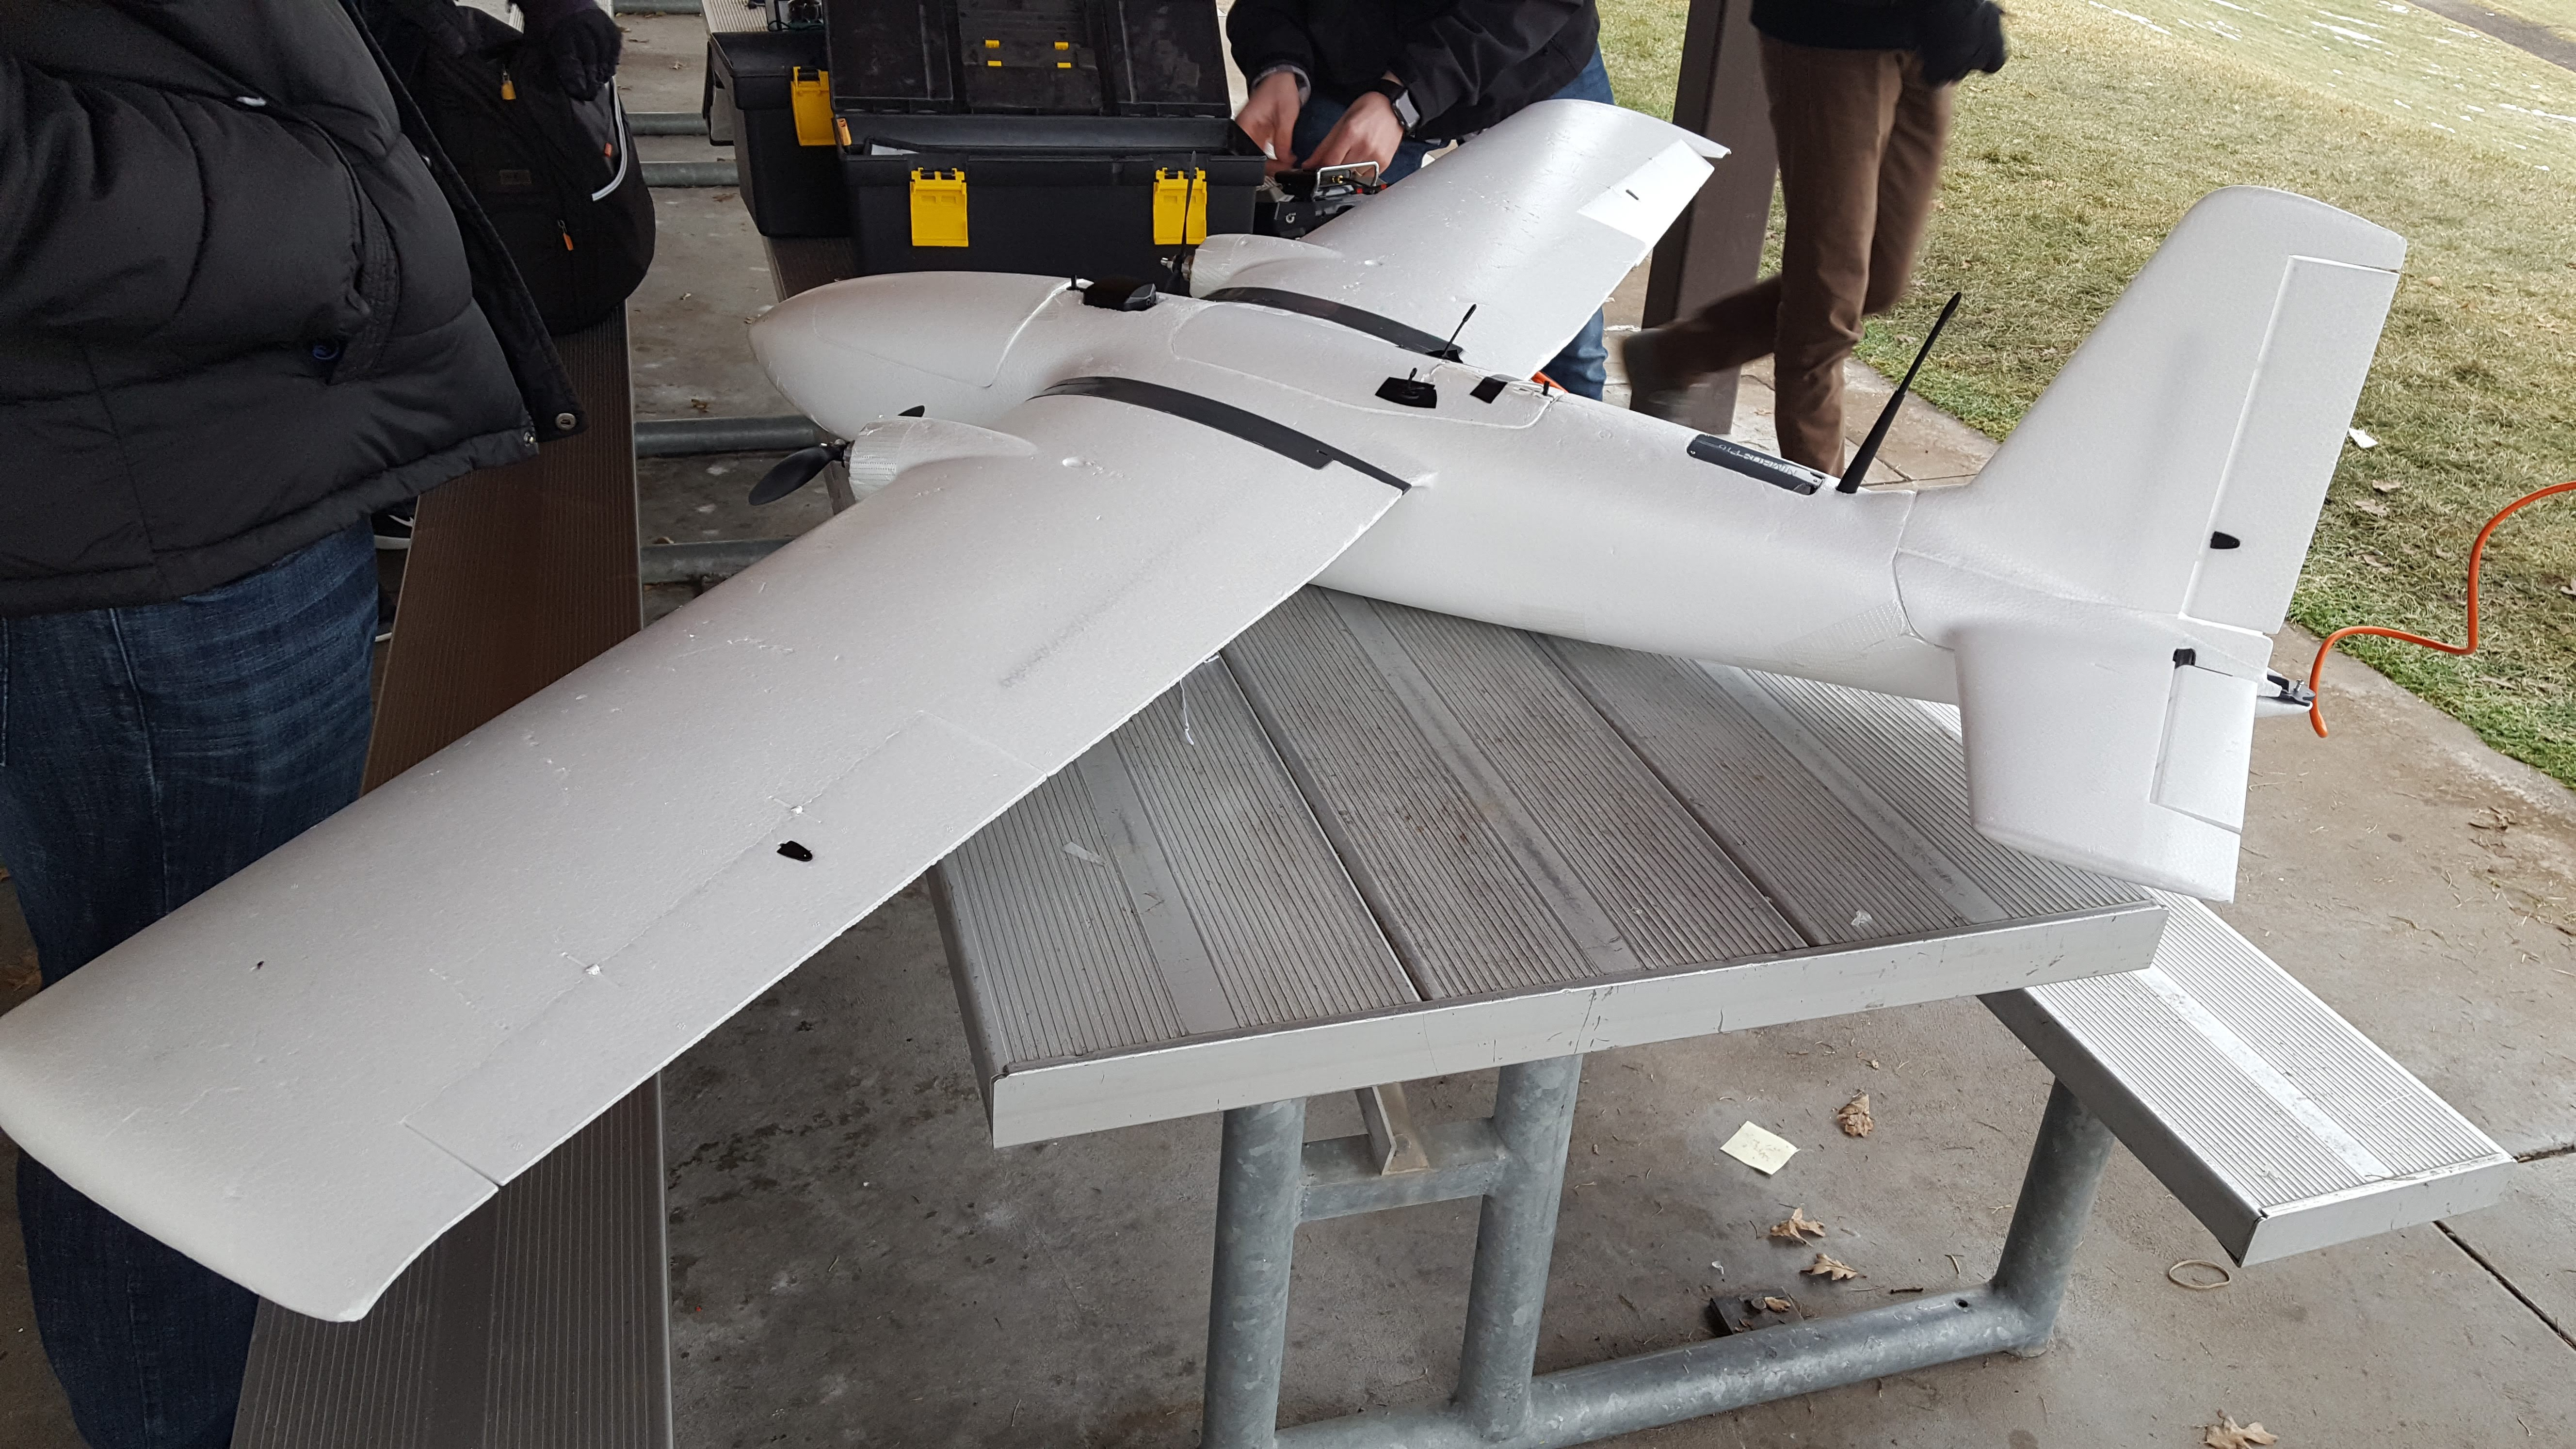
\includegraphics[width=.9\columnwidth]{figs/plane1}
	\caption{Fully-constructed Nimbus Pro airframe before its first flight.}
	\label{fig:plane1}
\end{figure} 

The full procedure for constructing the plane will not be outlined here, but it follows basic principles and steps that are used in almost every aircraft construction:

\begin{itemize}
	\item Glue fuselage sections together
	\item Attach proper servos and control horns to each control surface
	\item Attach motors and ESCs to wings
	\item Attach tail pieces
	\item Install all electronic hardware/wiring
	\item Ensure connectors and joints are properly secured and strengthened if necessary
	\item Attach/connect wings
\end{itemize}

The center of gravity (CG) was carefully planned for during construction to ensure it could be in its optimal location once all hardware was installed. The following modifications were made to our airframe based on our application and integrated hardware:

\begin{itemize}
	\item Holes were made in the main compartment hatch for the RC and Ubiquiti antennas to poke through. There is space further back in the plane for these components, but we wanted to move the CG as far forward as possible to achieve a desirable static margin. They were also placed so as to avoid interference with the GPS signal.
	\item The GPS slot on top was not used and taped over. The GPS was instead placed inside the nose of the plane to help with CG placement.
	\item The servos we used were a little larger than the original plane design anticipated. Because of this, some foam and plastic  needed to be cut away from servo locations to allow them to fit.
	\item A foam wedge was inserted underneath the tail to increase the tail incidence angle (see further details below).
	\item Small holes were drilled into the wing connector pieces to allow for the large wires to extend from the ESCs in the wings to the fuselage.
	\item In general, most components were placed as far forward as was reasonable to move our CG forward and increase our static margin. Doing so would help stabilize our plane and allow it to fly slower.
\end{itemize}

In Concept Development, we decided that we would try to modify our plane by adding wing extensions to increase total span. This would help the plane fly slower by reducing induced drag. Flying at a lower velocity would then help us achieve higher performance in our key success measures (specifically obstacles hit, waypoint proximity, characteristics identified, and accuracy of payload drop). In the process of building the plane and evaluating our timeline for this project, we've decided to forgo the wing extension modification. As described more in AF??, our airplane flies great without wing extensions, and any extra benefit to extensions would not be worth the time and effort required to design, implement and test these extensions.

One unanticipated modification we've made to the aircraft is the placement of a foam wedge underneath the tail of the plane. When modeling the Nimbus Pro, we were able to predict stable behavior and a high-performing aerodynamic efficiency (and thus a slower cruising velocity) for the airframe. These conclusions were predicated on a tail incidence angle of about -7 degrees. Upon getting the plane, we could not implement this angle without inserting a wedge beneath the tail to increase its incidence angle. At first, we decided to see if the plane did not need such a modification - it did fly, but it had a consistent tendency to want to pitch forward. This made it longitudinally unstable and difficult to manually fly. After installing the tail wedge, this problem was averted. The plane is now stable and flies at the design speed we had originally planned for.

The tail wedge (see Fig. \ref{fig:wedge}) is made out of extruded polystyrene, measured and cut manually in order to give the required incidence angle for the tail. Several notches were carved into the top for it to securely fit with the tail connector pieces. Fiber tape was then wrapped around it to ensure it would not come loose during flight. The design drawing for the wedge is in Artifact AF??.

\begin{figure}[h!]
	\centering
	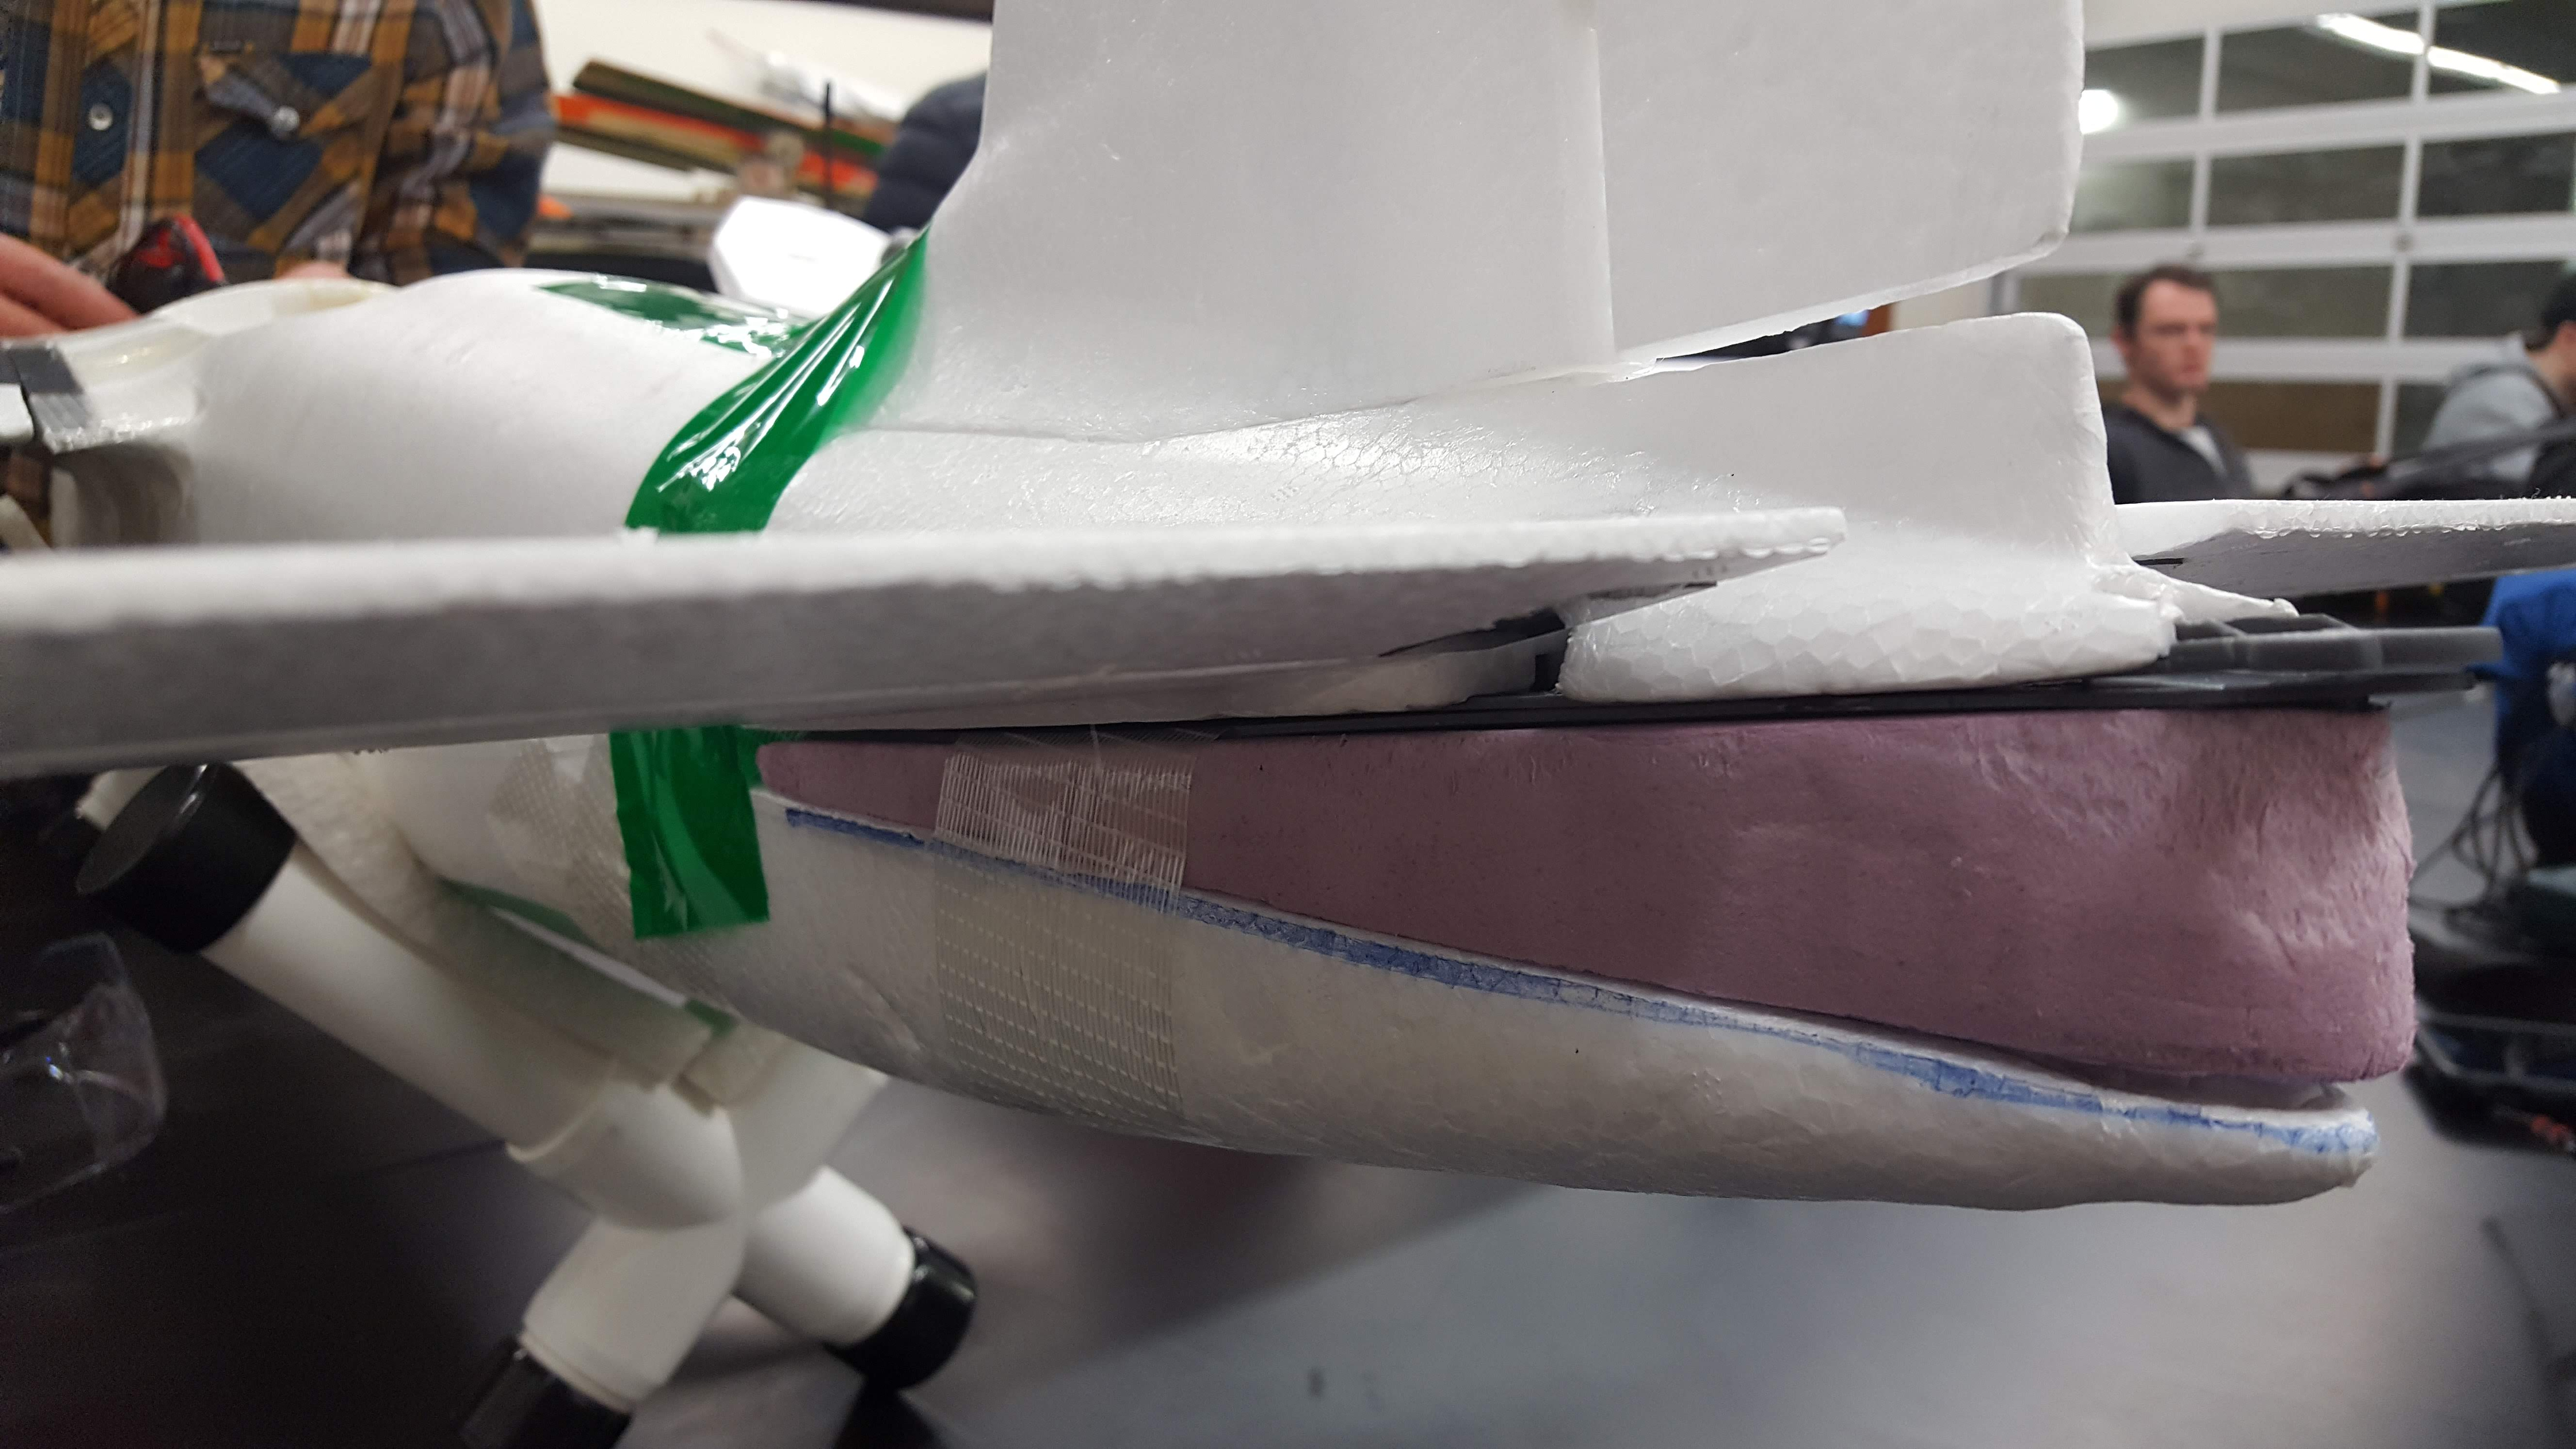
\includegraphics[width=.75\columnwidth]{figs/tailwedge}
	\caption{A foam tail wedge installed underneath the tail of the plane to increase its incidence angle and improve stability.}
	\label{fig:wedge}
\end{figure}

\section{Testing}
As described further in Artifact AF??, we have done extensive flight testing to ensure our airframe performs as expected. In the past couple of months, we have had several successful flight tests with manual RC control and multiple successful flights while controlling with autopilot. While flying, it is very stable and flies at an average of ~15\ m/s. These outcomes show that our airframe works and is very capable to integrate with the other subsystems. Not only have we flown it with some autopilot control, we have also shown it can hold the imaging subsystem camera and the UGV subsystem. Both have demonstrated their subsystems can work with the plane while stationary, and we have yet to test them in flight. From these results, however, we are very confident our airframe will integrate well with these subsystems while in flight. 

\section{Conclusion}
Our airframe is fully assembled (with slight modifications) and has proven to consistently fly reliably. All of our key success measures depend on the airframe flying well - and many of them can be improved if the airframe flies with a low velocity. Our design and modifications ensure the airframe does fly slowly, which will help minimize obstacles hit, waypoint proximity, and error when dropping the UGV payload. It also improves image quality to identify more characteristics. The plane has flown successfully with periodic autopilot control, and the UGV and imaging subsystems have performed well inside the plane while stationary. We fully expect all three other subsystems to successfully integrate with the airframe during flight.

\end{document}
